% The contents of this file is 
% Copyright (c) 2009-  Charles R. Severance, All Righs Reserved

\chapter{Por que você deveria aprender a programar?} %Vinícius

Escrever programas (ou programar) é uma atividade muito criativa e gratificante. Você pode escrever programas por várias razões, seja para ``ser seu ganha pão'' ou até para resolver problemas complexos de análises de dados ou apenas se divertir ajudando alguém a solucionar um problema. 
Este livro assume que \emph{todo mundo} precisa saber como programar, e, uma vez  sabendo, você vai descobrir o que deseja fazer com suas novas habilidades.

Em nosso dia-a-dia, estamos rodeados de computadores, sejam laptops, celulares, etc. Nós podemos imaginar esses computadores como nossos ``assistentes pessoais'', que cuidam de muitas de nossas coisas.

O \emph{hardware} dos nossos computadores cotidianos é essencialmente construído para nos perguntar continuamente: ``O que você deseja que eu faça agora?'' 

\centerline{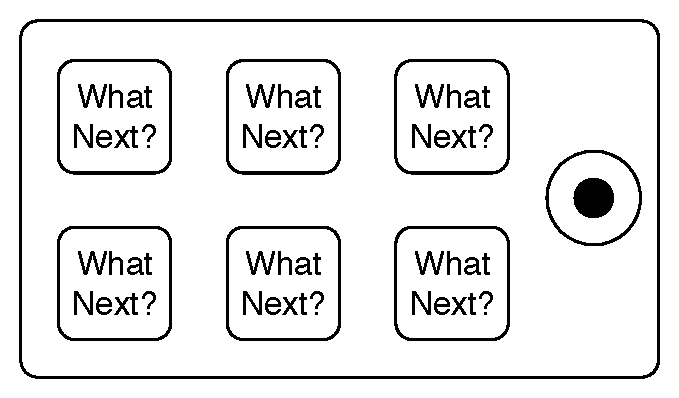
\includegraphics[height=1.00in]{figs2/pda.eps}}

Os programadores adicionam um sistema operacional e um conjunto de aplicativos ao \emph{hardware} e nós acabamos tendo um Assistente Pessoal Digital que é bastante útil e capaz de nos ajudar em várias coisas. 

Nossos computadores são rápidos e têm vastos espaços de memória e poderiam ser ainda mais úteis se nós {apenas} soubéssemos ``falar'' a língua para explicar ao computador o que nós ``queremos que ele faça agora''. Se nós soubéssemos essa linguagem, poderíamos mandar o computador realizar tarefas repetitivas ao nosso querer. Interessantemente, os tipos de coisas que computadores podem fazer de melhor são muitas vezes as coisas que nós humanos achamos entendiantes e mentalmente exaustivas.

Por exemplo, leia os três primeiros parágrafos desse capítulo e me diga qual é a palavra mais usada e quantas vezes essa mesma palavra apareceu. Enquanto você era capaz de ler e entender as palavras em poucos segundos, contar o número de vezes que a palavra foi usada é quase que doloroso, pois esse não é o tipo de problema que mentes humanas foram feitas para resolver. Para um computador é o contrário, ler e entender o texto escrito num pedaço de papel é difícil, mas contar as palavras e dizer quantas vezes aquela palavra foi usada é muito fácil:

\begin{verbatim}
python words.py
Enter file:words.txt
que 6
\end{verbatim}

Nosso ``assistente pessoal de análises de informação'' rapidamente nos diria que a palavra ``que'' foi usada seis vezes nos três primeiros parágrafos deste capítulo

Este mesmo fato de que computadores são bons em coisas que humanos não são é o motivo pelo qual você precisa se tornar hábil em falar a ``linguagem computacional''. Uma vez que você aprende essa nova linguagem, você pode designar tarefas mundanas para seu parceiro (o computador), sobrando mais tempo para fazer as coisas as quais é unicamente adequado. Você traz criatividade, intuição e inventividade a essa parceria.  
%%%%%%%%%%%%%%%%%%%%%%%%%%%%%%%%%%%%%%%%%%%%%%%%%%
\section{Criatividade e motivação} %Natã e maysa

Embora este livro não seja destinado a programadores profissionais, a programação profissional pode ser um trabalho muito gratificante, tanto financeiramente quanto pessoalmente. Construir programas úteis, elegantes e inteligentes para os outros usarem é uma atividade que exige muita criatividade. Seu computador ou Personal Digital Assistant (Assistente Pessoal Digital - PDA) geralmente contém diversos programas de diferentes grupos de programadores, cada um competindo por sua atenção e interesse. Eles fazem o melhor para atender às suas necessidades e lhe oferecer uma ótima experiência no processo. Em algumas situações, quando você escolhe um software, os programadores são diretamente compensados por sua escolha.

Se pensarmos nos programas como 
o resultado da criatividade de grupos de programadores, talvez a seguinte figura seja uma versão mais sensata de nosso PDA:


\centerline{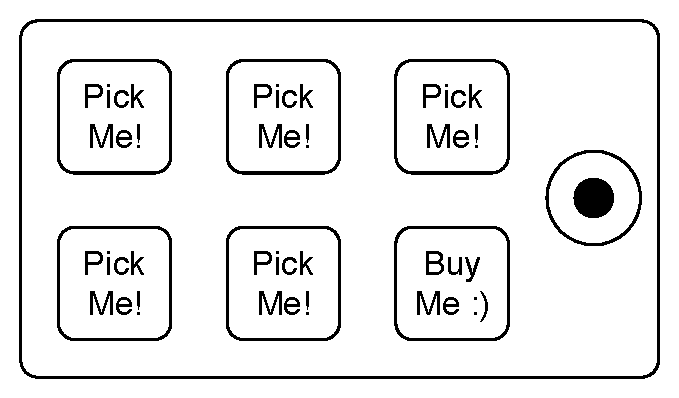
\includegraphics[height=1.00in]{figs2/pda2.eps}}


Por enquanto, nossa principal motivação não é ganhar dinheiro ou agradar os usuários finais, mas sim, sermos mais produtivos no manuseio dos dados e das informações que encontraremos em nossas vidas. Quando você começar, você será o programador e o usuário final de seus programas. À medida que você ganha experiência como programador e a programação lhe parece mais criativa, seus pensamentos podem se voltar ao desenvolvimento de programas para os outros.

%%%%%%%%%%%%%%%%%%%%%%%%%%%%%%%%%%%%%%%%%%%%%%%%%%
\section{Arquitetura de Hardware de Computadores}%João
\index{hardware}
\index{hardware!architecture}

Antes de começarmos a aprender a linguagem que usamos para dar instruções a computadores para o desenvolvimento de software, precisamos saber um pouco sobre como computadores são construídos. Se você por acaso desmontasse seu computador ou celular, encontraria as seguintes partes:


\centerline{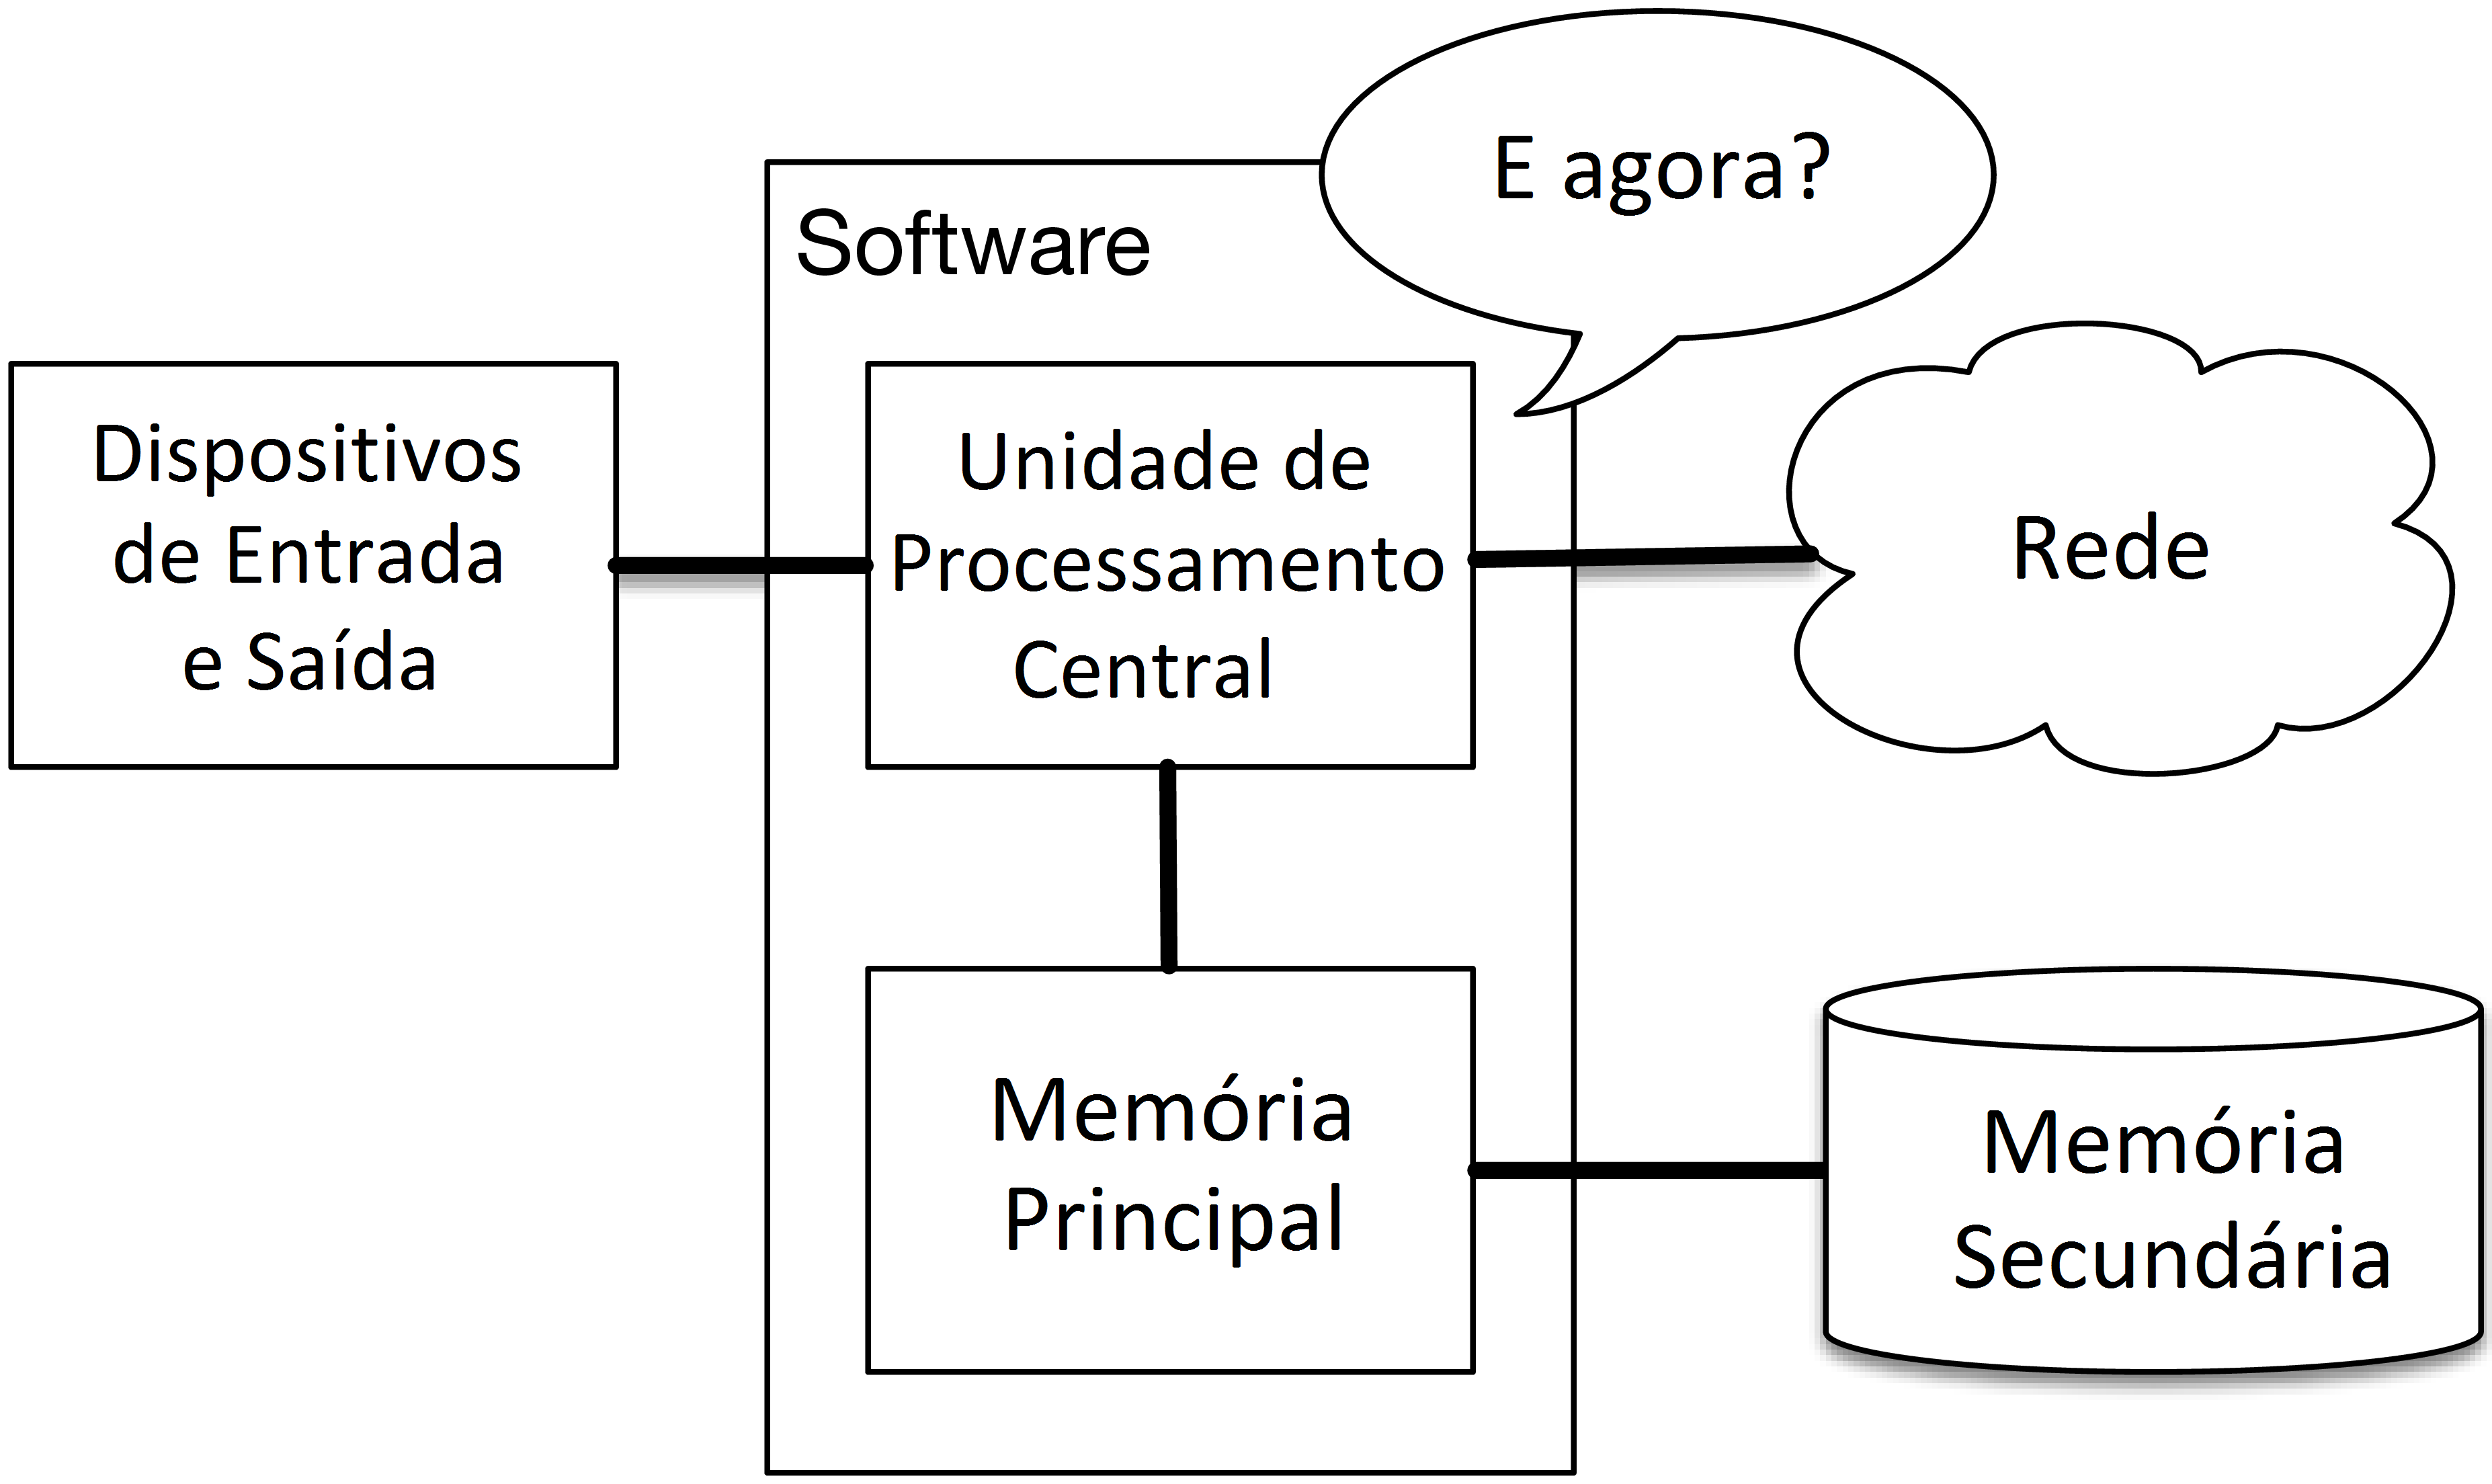
\includegraphics[height=2.50in]{imagens/arch.png}}


As definições em alto nível dessas partes são as seguintes:

\begin{itemize}
%Não sei se a melhor tradução de "What's next?" é "E agora?"
\item A {\bf Unidade de Processamento Central} (ou CPU) é a parte do computador que é construída para ser obcecada com a pergunta ``E agora?''.  Se seu computador é avaliado em 3.0 Gigahertz, significa que ele irá perguntar ``E agora?'' três bilhões de vezes por segundo. Você terá que aprender como falar rápido para acompanhar a CPU.
%Traduzi essa parte substituindo a palavra "main memory" para evitar repetições

\item A {\bf Memória Principal} é utilizada para armazenar informações que a CPU precisa com urgência. Sendo a memória quase tão rápida quanto a CPU. Mas a informação armazenada nessa memória desaparece quando o computador é desligado.
%Talvez exista uma melhor tradução para disk drive
\item A {\bf Memória Secundária} também é utilizada para armazenar informação, mas é muito mais lenta que a memória principal. A vantagem é que os dados podem ser guardados até quando o computador está desligado.  Exemplos de memória secundária são os discos rígidos ou as  memórias flash (tipicamente encontrados em dispositivos USB e reprodutores de música portáteis).

\item Os {\bf Dispositivos de Entrada e Saída} são simplesmente nosso monitor, mouse, microfone, alto-falante, touchpad, etc. Eles são todas as maneiras que temos para interagir com o computador.

\item Atualmente, a maioria dos computadores também tem uma
{\bf Conexão de rede} para receber informações de uma rede.
Podemos pensar nisso como um local muito devagar para armazenar e receber informação que podem nem sempre estar ``à disposição''.  Então, em resumo, essa rede é uma forma lenta e às vezes não confiável de {\bf Memória Secundária}.

\end{itemize}

Embora seja melhor deixar para construtores de computadores a maioria dos detalhes de como esses componentes funcionam, ter algumas terminologias ajuda uma vez que podemos falar dessas partes à medida que escrevemos nossos programas. 

Como um programador, seu trabalho é usar e orquestrar cada um desses recursos para resolver o problema que você precisa resolver e analisar as informações obtidas da solução.  Você vai, na maioria das vezes, estar ``falando'' com a CPU e dizendo a ela o que fazer agora. Algumas vezes dirá para usar a memória principal, memória secundária, rede, ou os dispositivos de entrada e saída.


\centerline{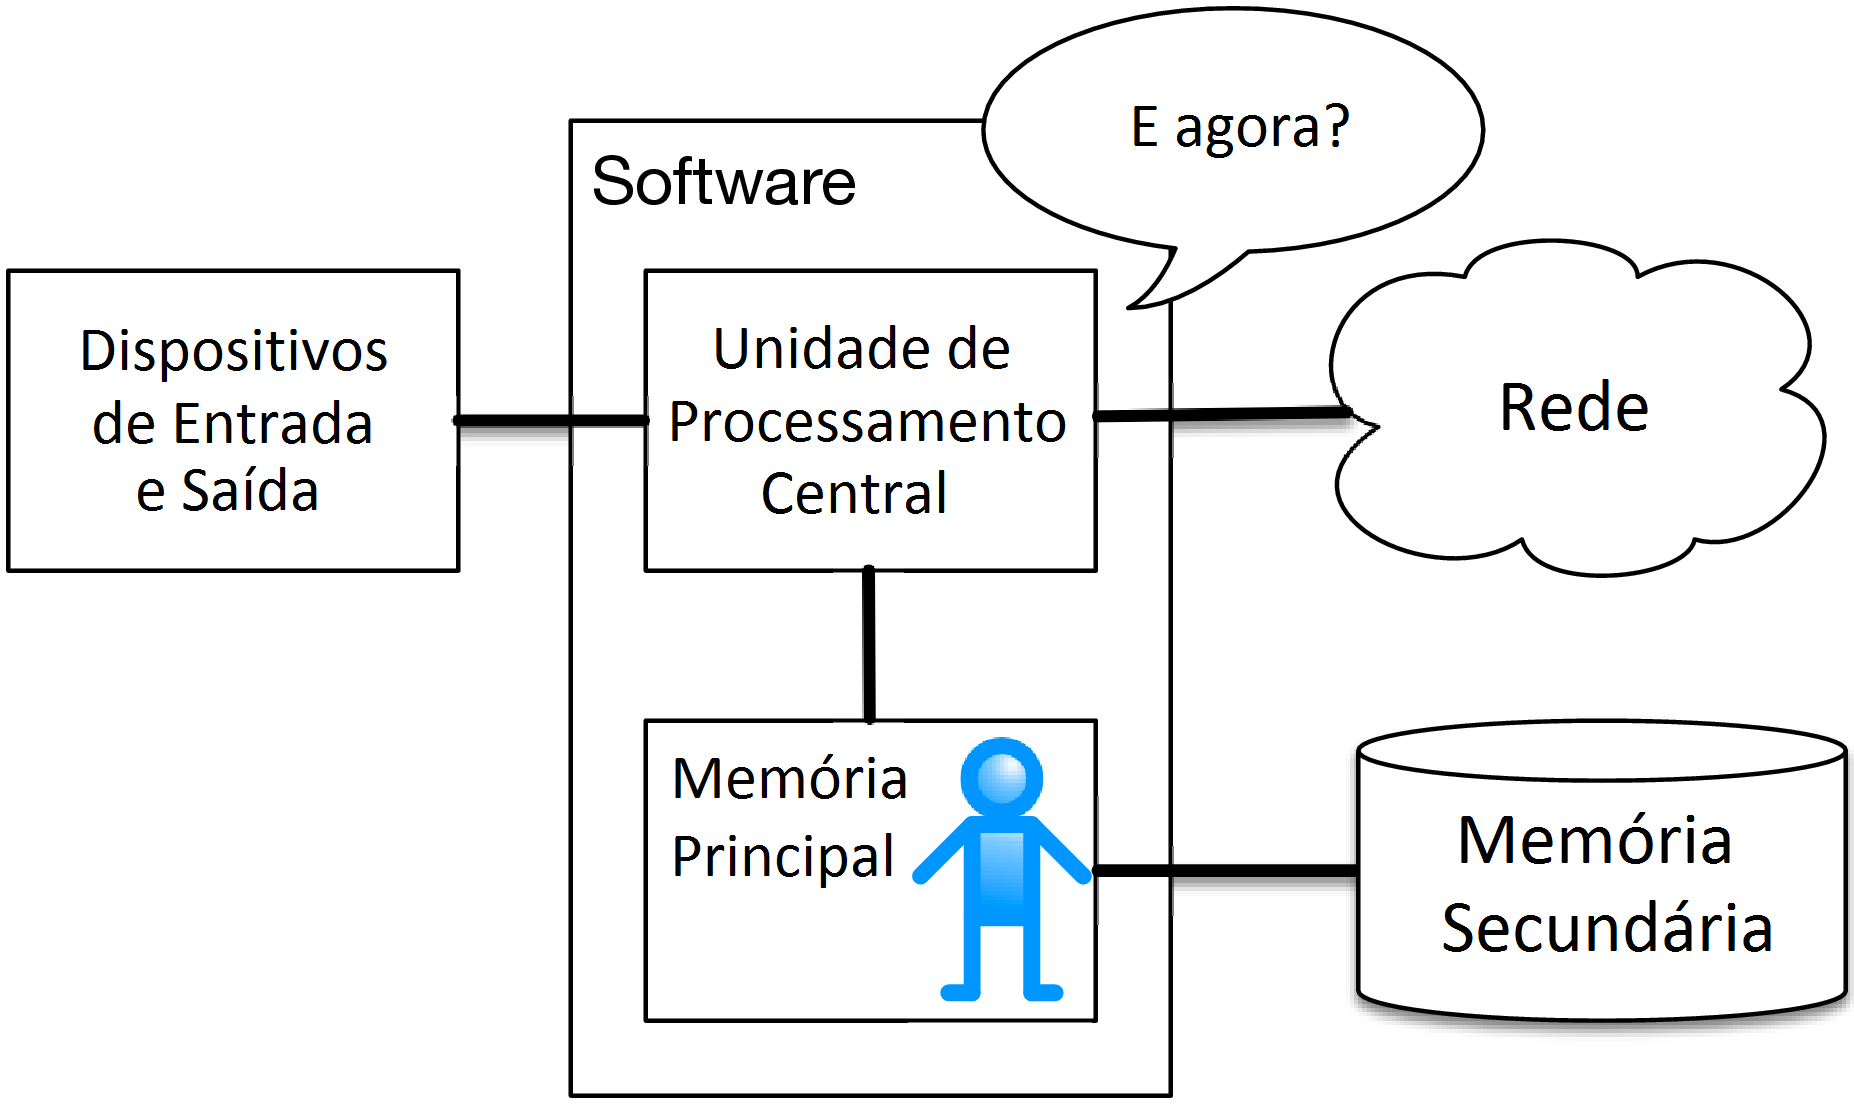
\includegraphics[height=2.50in]{imagens/arch2.png}}


Você precisa ser a pessoa que responde à pergunta ``E agora?'' da CPU.  Mas seria bem desconfortável te encolher a um tamanho de 5 mm só para que você emita um comando três bilhões de vezes por segundo.  Então, em vez disso, você deve escrever suas instruções antecipadamente.
Chamamos essas instruções armazenadas de  {\bf programa} e o ato de escrevê-las e garantir que estejam corretas de  {\bf programar}.
%"Inconfortável" ou desconfortável?
%%%%%%%%%%%%%%%%%%%%%%%%%%%%%%%%%%%%%%%%%%%%%%%%%%
\section{Entendendo a Programação} %Yuri
No resto do livro, nós tentaremos te transformar numa pessoa que tem habilidade na arte de programar. No final você será um {\bf programador} --- talvez não um profissional, mas ao menos você terá a capacidade de olhar um problema relacionado a dados e/ou informações e conseguirá desenvolver um programa que solucione o problema.

\index{Resolução de Problemas}%%%Como fazer

De um modo ou de outro você precisará de duas habilidades para ser programador:

\begin{itemize}
    \item Primeiro, você terá que aprender a linguagem de programação (Python), ou seja, você tem que saber o vocabulário e a gramática. Você tem que ser capaz de soletrar as palavras adequadamente nesta nova linguagem de forma a construir ``sentenças'' bem elaboradas.
    
    \item Segundo, você precisa ``contar uma história''. Quando se conta uma história se combina palavras e sentenças para se transmitir uma ideia ao leitor. Existe uma habilidade e uma arte na construção de uma história e a habilidade contá-la é aperfeiçoada quando se escreve e alguém avalia o seu trabalho dando um feedback sobre o mesmo. Na área de  programação, o nosso programa é a ``história'' e o problema que nós estamos querendo solucionar é a ``ideia''.
\end{itemize}

A partir do momento que você aprende uma linguagem de programação como Python, você terá muito mais facilidade em aprender uma segunda linguagem de programação como Javascript ou C++. A nova linguagem poderá ter gramática e vocabulário diferentes, mas as habilidades para resolver problemas serão as mesmas através de todas elas.

Você aprenderá o ``vocabulário'' e as ``sentenças'' de Python muito rápido. Será mais demorado para você aprender a escrever um programa coerente para solucionar um problema novo. Nós ensinamos programação assim como ensinamos a escrever. Nós começaremos lendo e explicando problemas, depois nós escreveremos programas simples e logo após vamos passar para programas cada vez mais complexos conforme o tempo for passando. Em algum ponto você ``encontrará sua musa'' e perceberá padrões por conta própria e verá mais claramente como pegar um problema e escrever um programa que o soluciona. Quando chegar neste ponto programar será um processo agradável e criativo.

Começaremos com o vocabulário e a estrutura dos programas em Python. Seja paciente, pois os exemplos te lembrarão como foi ler pela primeira vez.

%%%%%%%%%%%%%%%%%%%%%%%%%%%%%%%%%%%%%%%%%%%%%%%%%%
\section{Palavras e Frases } %Alysson
\index{programming language}
\index{language!programming}

Ao contrário das línguas humanas, o vocabulário Python é realmente muito pequeno.
Chamamos de "vocabulário" as palavras "reservadas". Estas são palavras com um significado muito especial para Python. Quando ele as vê em um programa, elas tem um e apenas um significado para Python. Posteriormente, você escreverá programas com suas palavras próprias que chamará de variáveis. Você terá uma grande liberdade na escolha de nomes para as suas variáveis, mas não será possível utilizar as palavras reservadas do Python como um nome para uma variável.

Ao treinarmos um cão, usamos palavras especiais como "senta", "fica" e "pega". Quando você fala com um cão e não utiliza alguma destas palavras reservadas, eles encaram você com uma reação questionável em seu rosto ate que você diga uma palavra reservada.  
por exemplo, se você diz, 
``Eu desejo que você corra para melhorar sua saúde'', 
o que a maioria dos cães ouve é,
``blah blah blah {\bf corra} blah blah blah blah.''
Isso porque ``corra'' é uma palavra reservada na liguagem canina. Muitos podem sugerir que a linguagem entre seres humanos e gatos não tem palavras reservadas\footnote{\url{http://xkcd.com/231/}}.

As palavras reservadas na língua onde os seres humanos falam com Python incluem o seguinte:


\begin{verbatim}
and       del       from      not       while    
as        elif      global    or        with     
assert    else      if        pass      yield    
break     except    import    print              
class     exec      in        raise              
continue  finally   is        return             
def       for       lambda     try
\end{verbatim}

%
É só isto, e ao contrário de um cachorro, Python já está completamente treinado.
Quando você diz `` Try'', ele vai tentar fazer o comando todas as vezes sem falhar.
Eventualmente iremos aprender essas palavras reservadas e como elas são usadas, mas por ora vamos nos concentrar no equivalente Python de \textit{``Speak ''} (na língua humana-à-cachorro).  A vantagem de pedir a ele para falar,
é que podemos até mesmo dizer-lhe o que ele deve falar, dando-lhe uma mensagem em citações:


\begin{verbatim}
print ('Olá mundo!')
\end{verbatim}


E até escrevemos nossa primeira frase sintaticamente correta de Python.
Nossa sentença começa com a palavra reservada {\bf Print} seguido
por uma sequência de texto de nossa escolha entre aspas simples. Este conjunto de caracteres pode ser acompanhado de aspas simples ou duplas, sem distinção do funcionamento da função. Entretanto, é interessante utilizar-se de aspas duplas para os casos em que seja necessário utilizar as aspas simples como um apóstrofo.

%1ª Semana de Trabalho
%%%%%%%%%%%%%%%%%%%%%%%%%%%%%%%%%%%%%%%%%%%%%%%%%%%%%%%%%%%%%%%%%%%%%%%%%%%%%%%%%%%%%%%%%%%%%%%%%%%%%%%%%%%%%%%%%%%%%%%%%%%%%%%%%%%%%%%%%%%%%%%%%%%%%%%%%%%%%%%%%%%%%%%%%%%%%%%%%%%%%%%%%%%%%%%%%%%%%%%%%%%%%%%%%%%%%%%%%%%%%%%%%%%%%%%%%%%%%%%%%%%%%%%%%%%%%%%%%%%%%%%%%%%%%%%%%%%%%%%%%%%%%%%%%%%%%%%%%%%%%%%%%%%%%%%%%%%%%%%%%%%%%%%%%%%%%%%%%%%%%%%%%%%%%%%%%%%%%%%%%%%%%%%%%%%%%%%%%%%%%%%%%%%%%%%%%%%%%%%%%%%%%%%%%%%%%%%%%%%%%%%%%%%%%%%%%%%%%%%%%%%%%%%%%%%%%%%%%%%%%%%%%%%%%%%%%%%%%%%%%%%%%%%%%%%%%%%%%%%%%%%%%%%%%%%%%%%%%%%%%%%%%%%%%%%%%%%%%%%%%%%%%%%%%%%%%%%%%%%%%%%%%%%%%%%%%%%%%%%%%%%%%%%%%%%%%%%%%%%%%%%%%%%%%%%%%%%%%%%%%%%%%%%%%%%%%%%%%%%%%%%%%%%%%%%%%%%%%%%%%%%%%%%%%%%%%%%%%%%%%%%%%%%%%%%%%%%%%%%%%%%%%%%%%%%%%%%%%%%%%%%%%%%%%%%%%%%%%%%%%%%%%%%%%%%%%%%%%%%%%%%%%%%%%%%%%%%%%%%%%%%%%%%%%%%%%%%%%%%%%%%%%%%%%%%%%%%%%%%%%%%%%%%%%%%%%%%%%%%%%%%%%%%%%%%%%%%%%%%%%%%%%%%%%%%%%%%%%%%%%%%%%%%%%%%%%%%%%%%%%%%%%%%%%%%%%%%%%%%%%%%%%%%%%%%%%%%%%%%%%%%%%%%%%%%%%%%%%%%%%%%%%%%%%%%%%%%%%%%%%%%%%%%%%%%%%%%%%%%%%%%%%%%%%%%%%%%%%%%%%%%%%%%%%%%%%%%%%%%%%%%%%%%%%%%%%%%%%%%%%%%%%%%%%%%%%%%%%%%%%%%%%%%%%%%%%%%%%%%%%%%%%%%%%%%%%%%%%%%%%%%%%%%%%%%%%%%%%%%%%%%%%%%%%%%%%%%%%%%%%%%%%%%%%%%%%%%%%%%%%%%%%%%%%%%%%%%%%%%%%%%%%%%%%%%%%%%%%%%%%%%%%%%%%%%%%%%%%%%%%%%%%%%%%%%%%%%%%%%%%%%%%%%%%%%%%%%%%%%%%%%%%%%%%%%%%%%%%%%%%%%%%%%%%%%%%%%%%%%%%%%%%%%%%%%%%%%%%%%%%%%%%%%%%%%%%%%%%%%% 
\section{Conversando com Python} %Vinícius França

Agora que nós já conhecemos uma palavra e uma simples sentença em Python, precisamos saber como iniciar uma conversa com ele para testar nossas novas habilidades linguísticas. 

Antes de você poder conversar com Python, você deve primeiro instalar o software do Python no seu computador e aprender a como inicializá-lo. Isso possui detalhes demais para este capítulo, então eu sugiro que você consulte \url{www.pythonlearn.com} onde eu tenho instruções detalhadas e vídeos sobre configuração e inicialização do Python nos sistemas Macintosh e Windows. Em certo ponto, você vai estar num terminal ou janela de comando e vai digitar {\bf python} e o interpretador de Python vai começar a executar no modo interativo, onde aparece algo como o seguinte:

\index{modo interativo}


\begin{verbatim}
Python 2.6.1 (r261:67515, Jun 24 2010, 21:47:49) 
[GCC 4.2.1 (Apple Inc. build 5646)] on darwin
Type "help", "copyright", "credits" or "license" for more information.
>>> 
\end{verbatim}

%
O {\tt >>>} ``prompt'' é o modo como o interpretador de Python te pergunta, ``O que você deseja que eu faça agora?'' Ele está pronto para ter uma conversa com você. Tudo o que você tem que saber é como falar a sua linguagem .

Vamos dizer, por exemplo, que você não conheça nem as mais simples palavras ou sentenças da linguagem Python. Você pode querer usar a frase padrão que os astronautas usam quando aterrissam num planeta distante e tentam falar com os habitantes locais:


\begin{verbatim}
>>> Venho em paz. Por favor, leve-me ao seu líder
  File "<stdin>", line 1
    Venho em paz. Por favor, leve-me ao seu líder
          ^
SyntaxError: invalid syntax (sintaxe inválida)
>>> 
\end{verbatim}

%
Isso não está indo muito bem. A menos que você pense em algo rápido, provavelmente os habitantes do planeta irão te apunhalar com suas lanças, colocarão você num espeto, te assarão sobre o fogo e comerão sua carne no jantar.

Felizmente, você levou uma cópia deste livro para sua viagem, abre ele nesta exata página e tenta de novo:

\begin{verbatim}
>>> print ('Alô Mundo!')
Alô Mundo!
\end{verbatim}

%
Isso está parecendo bem melhor, então você tenta se comunicar um pouco mais:


\begin{verbatim}
>>> print (`Você deve ser o lendário Deus que vem do céu')
Você deve ser o lendário Deus que vem do céu
>>> print (`Nós estávamos te esperando há um longo tempo')
Nós estávamos te esperando há um longo tempo
>>> print (`A lenda diz que você fica bastante saboroso com mostarda')
A lenda diz que você fica bastante saboroso com mostarda
>>> print `Nós teremos um banquete esta noite a menos que você diga
  File "<stdin>", line 1
    print `Nós teremos um banquete esta noite a menos que você diga
                                                                  ^
SyntaxError: Missing parentheses in call to 'print'
            (Falta de parênteses no uso de 'print')
>>> 
\end{verbatim}
%No livro original que eu tenho baixado em pdf, o erro nesse exemplo de cima não é o que está aí (EOL while...), e sim sobre o print não possuir parenteses, o que estaria errado. Quem puder, confira com a versão original que você tiver, por favor.

%
A conversa estava indo tão bem por um momento, até que você cometeu o menor erro na linguagem Python e ele pegou as lanças de volta. 

A essa altura, você também deve ter percebido que, enquanto Python é maravilhosamente complexo e poderoso e muito exigente sobre a sintaxe que você usa para se comunicar com ele, o mesmo {\em não} é inteligente. Você está apenas tendo uma conversa consigo mesmo, porém usando uma sintaxe apropriada.

De certo modo, quando você usa um programa escrito por outras pessoas, a conversa é entre você e esses outros programadores, com o Python atuando como intermediário. Ele é um meio pelo qual os criadores de programas expressam como a conversa deve proceder. E em alguns poucos mais capítulos, você será um desses programadores usando-o para conversar com os usuários do seu programa.

Antes de nós acabarmos nossa primeira conversa com o interpretador de Python, você provavelmente deve saber como, adequadamente, dizer ``good-bye", quando se está interagindo com os habitantes do planeta Python:

\begin{verbatim}
>>> good-bye
Traceback (most recent call last):
  File "<stdin>", line 1, in <module>
NameError: name 'good' is not defined (nome 'good' não está definido)

>>> if you don't mind, I need to leave
  File "<stdin>", line 1
    if you don't mind, I need to leave
             ^
SyntaxError: invalid syntax (sintaxe inválida)

>>> quit()
\end{verbatim}

%
Você irá perceber que os erros são diferentes para cada uma das tentativas falhas. O segundo erro é diferente porque {\bf if} é uma palavra reservada e o Python viu isso e pensou que estávamos tentando dizer algo, mas teríamos errado na sintaxe da frase.

A maneira certa se despedir do Python é inserir {\bf quit()} na parte interativa do {\tt >>>} prompt. Provavelmente, você teria demorado um pouco para adivinhar essa, então ter um livro em mãos será bem útil.

\section{Terminologia: interpretador e compilador}
Python é uma  linguagem de {\bf alto-nível} que pretende ser relativamente simples para um humano ler e escrever e para um computador ler e processar. Algumas outras linguagens de alto-nível são: Java, C++,
PHP, Ruby, Basic, Perl, JavaScript, and many more. O Hardware dentro da Unidade de Processamento Central (CPU) não entende nenhuma dessas linguagens de alto-nível.

A CPU entende uma linguagem que chamamos de {\bf linguagem de máquina}. Ela é muito simples e francamante bem cansativa de escrever, uma vez que é representada totalmente por zeros e uns.


\begin{verbatim}
01010001110100100101010000001111
11100110000011101010010101101101
...
\end{verbatim}

%
Linguagem de máquina parece ser bem simples superficialmente, visto que somente há zeros e uns, mas sua sintaxe é bem mais complexa e muito mais complicada que Python.  Então, poucos trabalhadores escrevem nessa linguagem. Em vez disso, construímos vários tradutores para permitir que programadores escrevam em linguagens de alto-nível, como Python ou JavaScript,
e esses tradutores convertem os programas para linguagem de máquina para a real execução pela CPU.

Uma vez que a linguagem de máquina está amarrada ao hardware do computador, ela não é {\bf portátil} para diferentes tipos de hardware. Programas escritos em linguagens de alto-nível podem ser movidos entre diferentes computadores usando um diferente interpretador na nova máquina ou recompilando o código para criar uma versão da linguagem de máquina para o novo computador.

Esses tradutores de linguagem de programação caem em duas categorias gerais:
(1) interpretadores e (2) compiladores.

Um {\bf interpretador} lê o código-fonte do programa como o programador escreveu, analisa o código e interpreta as instruções em tempo real.
%%Aqui adaptei um pouco visto a repetição excessiva da palavra Python, que não cai muito bem no português
Python é um interpretador e quando estamos executando Python interativamente, podemos digitar uma linha (uma sentença) e ela é processada imediatamente e já podemos digitar outra linha de Python.   

Algumas das linhas de Python falam para ele que você quer aquilo para lembrar de algum valor para depois. Precisamos escolher um nome para esse valor que será lembrado e podemos usar esse nome simbólico para recuperar o valor depois. Usamos o termo {\bf variável} para nos referir a esses rótulos que se referem à informação armazenada.


\begin{verbatim}
>>> x = 6
>>> print (x)
6
>>> y = x * 7
>>> print (y)
42
>>> 
\end{verbatim}

%
Nesse exemplo, pedimos para o Python que lembre o valor seis e use o rótulo {\bf x} para que possamos recuperar o valor depois. Nós verificamos que ele realmente lembrou o valor usando {\bf print}. Então, pedimos que o interpretador recupere {\bf x} e multiplique por sete, colocando o valor recentemente computado em {\bf y}. Então, pedimos ao Python para mostrar o valor que está atualmente em {\bf y}.

Apesar de escrevermos esses comandos em Python uma linha por vez, ele trata os comandos como uma sequência ordenada de afirmações com afirmações posteriores capazes de recuperar informações criadas em afirmações anteriores.  Estamos escrevendo nosso primeiro parágrafo simples com quatro sentenças em uma ordem lógica e significativa.

É da natureza de um {\bf interpretador} ser capaz de ter uma conversa interativa como mostrada acima. Um {\bf compilador} precisa receber todo o programa em um arquivo, e então executa um processo para traduzir o código-fonte de alto-nível para linguagem de máquina e então o compilador põe a linguagem de máquina resultante em um arquivo para posterior execução.

Se você possui um sistema Windows, frequentemente esses programas executáveis em linguagem de máquina têm um sufixo ``.exe'' ou ``.dll'' que correspondem a ``executável'' e ``biblioteca de vínculo dinâmico'' respectivamente.  No Linux e Macintosh, não há sufixo que marque exclusivamente um arquivo como executável.

Se você for abrir um arquivo executável em um editor de texto, ele vai parecer completamente louco e será ilegível.


\begin{verbatim}
^?ELF^A^A^A^@^@^@^@^@^@^@^@^@^B^@^C^@^A^@^@^@\xa0\x82
^D^H4^@^@^@\x90^]^@^@^@^@^@^@4^@ ^@^G^@(^@$^@!^@^F^@
^@^@4^@^@^@4\x80^D^H4\x80^D^H\xe0^@^@^@\xe0^@^@^@^E
^@^@^@^D^@^@^@^C^@^@^@^T^A^@^@^T\x81^D^H^T\x81^D^H^S
^@^@^@^S^@^@^@^D^@^@^@^A^@^@^@^A\^D^HQVhT\x83^D^H\xe8
....
\end{verbatim}

%
Não é fácil ler ou escrever em linguagem de máquina, então é ótimo termos os 
{\bf interpretadores} e {\bf compiladores} que nos permitem escrever em linguagens de alto-nível como Python ou C.

Agora, a esse ponto de nossa discussão de compiladores e interpretadores, você deveria estar se perguntando um pouco sobre o interpretador Python em si. Em qual linguagem ele é escrito? Ele é escrito em uma linguagem compilada? Quando nós digitamos ``python'', o que está exatamente acontecendo?

O interpretador Python é escrito em uma linguagem de alto-nível chamada C. Você pode dar uma olhada no código-fonte real do interpretador Python indo em \url{www.python.org} e trilhando seu caminho pelo código-fonte. and working your way to their source code.
Então, Python é propriamente um programa e é compilado em código de máquina.
Quando você instalou o Python no seu computador (ou o fornecedor instalou), você copiou uma cópia de um código de máquina do programa Python traduzido no seu sistema.   No Windows, o código de máquina executável para o Python em si está provavelmente em um arquivo com um nome do tipo:


\begin{verbatim}
C:\Python27\python.exe
\end{verbatim}

%
Isso é mais do que você realmente precisa saber para ser um programador de Python, mas às vezes vale a pena responder a essas perguntas irritantes logo no começo.

\section{Escrevendo um Programa}% Yuri
Escrever comandos no Interpretador de Python é uma grande forma de experimentar os recursos da linguagem, mas não é recomendado para resolução de problemas complexos. 

Quando queremos escrever um programa, 
nós utilizamos um editor de texto para escrever as instruções em Python no arquivo, isto é chamado de um {\bf script}. Por convenção, scripts em Python possuem nomes que terminam com {\tt .py}.


\index{script}
Para executar o script, você fala ao interpretador de Python o nome do arquivo. Em uma janela em Unix ou Windows, você escreveria  {\tt python alo.py} como a seguir:


To execute the script, you have to tell the Python interpreter 
the name of the file.  In a Unix or Windows command window, 
you would type {\tt python Alo.py} as follows:


\begin{verbatim}
\$ cat Alo.py
print ({ \color{blue}'Alô Mundo!'}) %Concertar a cor 
\$ python Alo.py
Alô Mundo!
\$
\end{verbatim}

%

O ``\$''  é o prompt do sistema operacional, e o ``cat Alo.py'' nos mostra que um arquivo ``Alo.py'' contém um programa em Python em uma linha que imprime uma string.

Nós chamamos o interpretador de Python e falamos com ele para que leia o código fonte do arquivo  ``Alo.py'' ao invés em vez de nos pedir linhas de código Python.

Você notará que não há necessidade de {\bf quit ()} no final do programa em Python. Quando o Python está lendo seu código-fonte
a partir de um arquivo, ele sabe parar quando chega ao final do arquivo.


\section{O que é um programa?} %Natã e Maysa

A definição de um  {\bf programa} em seu básico é uma sequência de instruções do Python que foram criadas para fazer algo. Até mesmo nosso simples  {\bf Alo.py} script é um programa. Trata-se de um programa de uma única linha e particularmente não é útil, mas na definição mais estrita, é sim um programa em Python.

Pode ser mais fácil entender o que é um programa pensando em um problema que um programa poderia ser criado para resolver, e então olhar para um que solucionaria este problema.

Digamos que você está fazendo uma pesquisa de Computação Social em posts do Facebook e que você está interessado nas palavras mais usadas frequentemente em uma série de posts. Você poderia imprimir o conteúdo dos posts do Facebook e examinar o texto procurando pela palavra mais comum, mas isso levaria muito tempo e seria muito propenso a erro. Você seria esperto escrevendo um programa em Python para lidar com esta tarefa rápida e precisamente então você passaria o fim de semana fazendo algo divertido.

Por exemplo, veja o seguinte texto sobre um palhaço e um carro. Veja o texto e descubra qual é a palavra mais comum e quantas vezes aparece.


\begin{verbatim}
O palhaço correu atrás do carro e o carro entrou na tenda e a 
tenda caiu sobre o palhaço e o carro. 
\end{verbatim}

%
Imagine então que você está fazendo essa tarefa olhando para milhões de linhas de texto. Francamente seria mais rápido para você aprender Python e escrever um programa nesta linguagem para contar as palavras do que seria examinar manualmente as palavras.

A notícia melhor ainda é que eu já escrevi um programa simples para encontrar a palavra mais comum em um arquivo de texto. Eu escrevi, testei, e agora estou lhe dando para você usar e economizar algum tempo.


\begin{verbatim}
name = raw_input('Inserir Arquivo:')
handle = open(name, 'r')
text = handle.read()
words = text.split()
counts = dict()

for word in words:
   counts[word] = counts.get(word,0) + 1

bigcount = None
bigword = None
for word,count in counts.items():
    if bigcount is None or count > bigcount:
        bigword = word
        bigcount = count

print ('bigword, bigcount')
\end{verbatim}

%
Você nem mesmo precisa saber  Python para usar este programa. Você irá precisar passar do Capítulo 10 desse livro para entender completamente as impressionantes técnicas de Python que nós usamos para fazer esse programa. Você é o usuário final, você simplesmente usa o programa e se maravilha com sua inteligência e como isso poupou você de muito esforço manual.
Você simplesmente digita o código em um arquivo chamado {\bf words.py} e  executa ou faz o download do código fonte de \url{http://www.pythonlearn.com/code/} e o executa.

\index{program}
Este é um bom exemplo de como Python e a Linguagem Python estão atuando como intermediário entre você (o usuário final) e eu (o programador).  Python é uma forma para nós trocarmos sequências de instruções úteis (i.e., programas) em uma linguagem comum que pode ser usada por qualquer um que o instale em seu computador. Então nenhum de nós está falando {\em com Python},
ao invés disso estamos nos comunicando {\em através dele}.

\section{The building blocks of programs} %Yuri

Nos próximos capítulos nós iremos aprender sobre vocabulário, estrutura de sentenças, pará-grafos e a estrutura da história de Python. Nós aprenderemos sobre a poderosa capacidade de Python e como integrar essas capacidades em conjunto para criar programas eficientes. 
%Coloquei um - em parágrafo para evitar um erro no latex na devida linha

Existem alguns padrões conceituais de baixo nível que usamos para construir programas. Essas construções não são apenas para programas em Python, elas fazem parte de todas as linguagens de programação, desde a linguagem da máquina até as linguagens de alto nível.   

\begin{description}

\item[entrada (input):] Obter dados do ``mundo externo''. Isso pode ser ler dados de um arquivo, ou até de algum tipo de sensor como um microfone ou GPS. Nos nossos programas iniciais, nossa entrada virá do usuário digitando dados do seu teclado.
\item[saída (output):] Mostrar  resultados de um programa numa tela, ou guarde-os em um arquivo, ou talvez gravá-los em um dispositivo como um alto falante, para que ele toque música ou fale algum texto.
\item[execução sequencial:] Realizar instruções uma após a outra na ordem na qual são encontradas no script
\item[execução condicional:] Checar por certas condições para que uma certa sequencia de instruções seja executada ou ignorada.
\item[execução repetitiva:] Realizar algum conjunto de instruções repetidamente, geralmente com alguma variação. 
\item[reuso:] Escrever um conjunto de instruções dando-se um nome para ele para que estas instruções sejam reutilizadas como necessários durante o programa.

\end{description}

Parece quase simples demais para ser verdade, e é claro que nunca é tão simples. É como dizer que andar é simplesmente "colocar um pé na frente do outro". A ``arte" de escrever um programa é compor e tecer esses elementos básicos juntos muitas vezes para produzir algo que é útil para seus usuários.

O programa de contagem de palavras acima usa diretamente todos os conceitos acima, exceto um.

\section{O que poderia dar errado?} %Alysson

Como vimos em nossas primeiras conversas com Python, devemos comunicar precisamente quando escrevemos o código em Python. O melhor desvio ou erro fará com que Python desista de olhar para o seu programa.

Os programadores iniciantes costumam ter o fato de que Python não deixa espaço para erros como prova de que ele é mau, odioso e cruel. Enquanto Python parece gostar de todos os outros, ele os conhece pessoalmente e guarda rancor contra eles.  Por causa desse rancor, Python leva nossos programas perfeitamente escrito e rejeitá-los como ``impróprios'' só para nos atormentar.


\begin{verbatim}
>>> print 'Olá Mundo!'
  File "<stdin>", linha 1
    print 'Ola mundo!'
                       ^
Erro de sintaxe: sintaxe inválida 
>>> primt 'Ola mundo '
  File "<stdin>", linha 1
    primt 'Ola mundo '
                      ^
Erro de sintaxe: sintaxe inválida
>>> Eu te odeio Python!
  File "<stdin>", line 1
    Eu te odeio Python!
         ^
Erro de sintaxe: sintaxe inválida
>>> Se você sair de lá, eu lhe ensinaria uma lição
  File "<stdin>", line 1
    Se você sair de lá, eu lhe ensinaria uma lição
              ^
Erro de sintaxe: sintaxe inválida
>>> 
\end{verbatim}

%
Há pouco a ser ganho por discutir com Python.  É apenas uma ferramenta.
Ele não tem emoções e é feliz e pronto para atendê-lo sempre que você
Preciso dele.  Suas mensagens de erro soam ásperas, mas eles são apenas um pedido de ajuda.  Ele olhou para o que você digitou, e simplesmente não pôde entender o que você inseriu.

Python é muito mais como um cão, amando-o incondicionalmente, tendo alguns
Palavras-chave que ele entende, olhando para você com um olhar doce em sua
Cara ({\tt >>>}), e esperando que você diga algo que ele compreenda.
Quando Python diz ``Erro de sintaxe: sintaxe inválida'', é simplesmente abanando
sua cauda e dizendo: ``você parecia dizer alguma coisa, mas eu simplesmente não entendi o que você quis dizer, mas por favor continue falando comigo ({\tt >>>}).''

Como seus programas se tornam cada vez mais sofisticados, você vai encontrar três 
tipos gerais de erros:

\begin{description}

\item[Syntax errors:] Estes são os primeiros erros que você vai fazer e os mais fáceis
para corrigir.  Um erro de sintaxe significa que você violou as regras ``gramática'' do Python. Assim, ele faz o seu melhor para apontar diretamente para a linha e caractere que ele percebeu estar confuso. A única complicação nos erros de sintaxe é que às vezes o erro se encontra na verdade um pouco antes de onde ele havia {\em notado} que estava confuso. Assim, a linha e caractere que o Python indica pode ser apenas o ponto de partida de sua investigação

\item[Logic errors:] Um erro lógico é quando o programa tem uma boa sintaxe, mas há um erro na ordem das afirmações ou talvez um erro na forma como as afirmações se relacionam entre si. UM bom exemplo de um erro lógico pode ser,  ``tomar uma bebida de sua garrafa de água, colocá-lo em sua mochila, caminhe até a biblioteca e, em seguida, coloque a parte de cima para trás na garrafa.''

\item[Semantic errors:]


Um erro semântico é quando a descrição dos passos a serem tomados é sintaticamente perfeita e na ordem certa, mas há um erro no programa. Ele está perfeito, mas não faz o que você pretendia que fizesse. Um exemplo simples seria
se você estivesse dando a uma pessoa direções para um restaurante e dissesse: ``... quando você chegar no cruzamento com o posto de gasolina, vire à esquerda e vá uma milha de distância e o restaurante é um edifício vermelho à sua esquerda.''  Seu amigo está muito atrasado e te chama para dizer que eles estão em uma fazenda e andando por trás de um celeiro, sem sinal de um restaurante.  
Então você diz ``você virou à esquerda ou direita no posto de gasolina?'' e 
Ele diz, ``Eu segui suas direções perfeitamente, eu as escrevi todas: diz para virar à esquerda e seguir uma milha em direção ao posto de gasolina.''  Então você diz, ``Eu sinto muito, porque enquanto minhas instruções foram sintaticamente corretas, elas infelizmente continha um erro semântico pequeno, mas não detectado.''

\end{description}

Novamente em todos os três tipos de erros,Python está tentando ao máximo fazer exatamente o que você pediu.

\section{Debugging} %Vinícius

Quando seu Python emite um erro ou até mesmo quando ele te dá um resultado diferente do esperado, você inicia a ``caça’’ em busca da causa de tal problema. ``{\it Debugging}’’ é o processo de encontrar essa causa em seu código. Quando você está fazendo o {\it Debugging} em seu programa, especialmente se for um erro difícil de encontrar, existem quatro coisas a se tentar: \\
\index{debugging} \\
%Não sei formatar como o original
{\bf  Ler:} Leia seu código. Fale-o em voz alta para si próprio e verifique se ele diz mesmo o que você quer que ele diga.

{\bf  Testar:} Experimente fazer mudanças e rodar diferentes versões do seu programa. Geralmente, quando você coloca a coisa certa no lugar certo, o problema se torna óbvio, porém, às vezes, você terá que gastar mais tempo para desvendá-lo.

{\bf  Refletir:} Tire um tempo para pensar! Que tipo de erro está acontecendo: sintaxe, semântica, em tempo de execução? Que informações você pode extrair das mensagens de erro, ou da saída do programa? Que tipo de erro poderia causar o problema que você está vendo? Qual foi a última coisa que você alterou antes do problema aparecer?

{\bf Retroceder:} Em certo momento, o melhor a se fazer é voltar atrás. Desfazer mudanças recentes, até retornar a um programa que funcione e que você o entenda. Depois você pode começar a reconstruir o código.\\

Programadores iniciantes às vezes ficam emperrados em uma dessas atividades e acabam esquecendo as outras. Para encontrar um erro complexo é preciso ler, testar, refletir e retroceder. Se você ficar preso em uma dessas, tente as outras. Cada uma corresponde a um estilo de problema diferente.

\index{erro tipográfico}
Por exemplo, ler seu código pode ajudar caso o problema seja um erro tipográfico, mas não se ele for uma má compreensão conceitual. Se você não entende o que o programa faz, você pode lê-lo 100 vezes e nunca verá o erro, porque o erro está na sua cabeça.

\index{debugging experimental }
Testar diferentes versões pode ajudar, principalmente se forem testes simples e pequenos. Po-rém, se você faz os testes sem pensar ou ler o seu código, você pode enquadrar-se num padrão que eu chamo de “programação randômica”, que é a arte de fazer mudanças aleatórias até que seu programa funcione da maneira certa. Obviamente, programação randômica pode lhe custar um bom tempo.
\index{random walk programming}

\index{development plan!random walk programming}
Você precisa tirar um tempo para pensar. {\it Debugging} é uma ciência experimental. Você deveria ter ao menos hipóteses sobre o que é o problema. Se existem duas ou mais possibilidades, tente pensar em um teste que eliminaria uma dessas.

Tirar uma folga ajuda no pensar. Pratique o falar também. Se você explicar o problema para outra pessoa (ou mesmo para si próprio), você às vezes encontrará a resposta antes de terminar a pergunta.

Mas até mesmo as melhores técnicas de {\it Debugging} irão falhar se houverem muitos erros, ou se o código que você está tentando concertar for muito grande e complicado. Às vezes, o melhor a se fazer é retroceder, simplificando o programa até que você retorne a algo que funcione e que você entenda.

A maioria dos programadores iniciantes são relutantes a retroceder, porque eles não suportam o fato de deletar uma linha de código (mesmo se estiver errada). Se isso te fizer se sentir melhor, copie seu código em outro arquivo antes de começar a desmontá-lo. Dessa maneira, você pode colar as peças de volta em pouquíssimo tempo.


\section{A jornada do aprendizado} %Andhré

Conforme for progredindo sobre os tópicos abordados no restante do livro, não deixe se abalar se sentir que os conceitos não estão fixando perfeitamente na primeira tentativa. Quando você está aprendendo a falar uma língua nova, não é um problema que os seus primeiros anos de prática não passem além do que singelas tentativas gorgolejantes. E está tudo em ordem se você leva um semestre apenas para evoluir de um vocabulário simples para pequenas sentenças, e se levar anos para transformar estas sentenças em parágrafos, e alguns anos a mais para conseguir escrever uma pequena fábula interessante com suas próprias palavras.

Nosso objetivo é que você aprenda Python de uma maneira muito mais rápida, por isso ensinamos tudo simultaneamente ao longo dos próximos capítulos. Todavia, é como aprender uma nova língua que leva um certo tempo para absorver e compreender antes que a sinta natural. Isto pode causar uma desorientação conforme visitamos e revisitamos alguns tópicos com o intuito de lhe fazer observar aquilo de uma visão macroscópica, isto enquanto estamos definindo uma pequena fração do que compõe o imenso todo. Ao passo que o livro for se desenvolvendo linearmente, e se você está cursando a disciplina ela também irá progredir linearmente, não hesite de abordar o material de uma maneira completamente diferente e não-linear. Leia coisas do começo ao fim, de acordo com sua necessidade e curiosidade. Ao ler de relance tópicos mais avançados, mesmo sem compreendê-los bem detalhadamente, você pode chegar à um entendimento melhor do ``por que?'' da programação. Ao revisar o material prévio, e até refazendo exemplos anteriores, você perceberá que na verdade houve um grande aprendizado sobre o material mesmo que o material estudado atualmente pareça um pouco impenetrável.

Usualmente, quando você está aprendendo sua primeira linguagem de programação, existem alguns momentos maravilhosos de ``Ah Hah!'', onde você pode se afastar e observar com um martelo e formão nas mãos que o pedaço de pedra que você está trabalhando, está se transformando numa escultura encantadora.

Se algumas vezes a tarefa de programar parecer ser particularmente difícil, não existe vantagem alguma em permanecer a noite em claro encarando o problema. Pare, relaxe, coma alguma coisa, explique o problema verbalmente com alguma pessoa(ou até mesmo o seu cachorro), e somente depois retorne a ele com uma nova perspectiva. Eu lhe garanto que no momento em que você compreender os conceitos de programação presentes neste livro, poderá olhar para trás e observar como tudo isto era realmente fácil e elegante, e que precisou apenas de um pouco do seu esforço e tempo para que tudo pudesse ser absorvido.
%%%%%%%%%%%%%%%%%%%%%%%%%%%%%%%%%%%%%%%%%%%%%%%%%%%%%%%%%%%%%%%%%%%%%%%%%%%%%%%%%%%%%%%%%%%%%%%%%%%%%%%%%%%%%%%%%%%%%%%%%%%%%%%%%%%%%%%%%%%%%%%%%%%%%%%%%%%%%%%%%%%%%%%%%%%%%%%%%%%%%%%%%%%%%%%%%%%%%%%%%%%%%%%%%%%%%%%%%%%%%%%%%%%%%%%%%%%%%%%%%%%%%%%%%%%%%%%%%%%%%%%%%%%%%%%%%%%%%%%%%%%%%%%%%%%%%%%%%%%%%%%%%%%%%%%%%%%%%%%%%%%%%%%%%%%%%%%%%%%%%%%%%%%%%%%%%%%%%%%%%%%%%%%%%%%%%%%%%%%%%%%%%%%%%%%%%%%%%%%%%%%%%%%%%%%%%%%%%%%%%%%%%%%%%%%%%%%%%%%%%%%%%%%%%%%%%%%%%%%%%%%%%%%%%%%%%%%%%%%%%%%%%%%%%%%%%%%%%%%%%%%%%%%%%%%%%%%%%%%%%%%%%%%%%%%%%%%%%%%%%%%%%%%%%%%%%%%%%%%%%%%%%%%%%%%%%%%%%%%%%%%%%%%%%%%%%%%%%%%%%%%%%%%%%%%%%%%%%%%%%%%%%%%%%%%%%%%%%%%%%%%%%%%%%%%%%%%%%%%%%%%%%%%%%%%%%%%%%%%%%%%%%%%%%%%%%%%%%%%%%%%%%%%%%%%%%%%%%%%%%%%%%%%%%%%%%%%%%%%%%%%%%%%%%%%%%%%%%%%%%%%%%%%%%%%%%%%%%%%%%%%%%%%%%%%%%%%%%%%%%%%%%%%%%%%%%%%%%%%%%%%%%%%%%%%%%%%%%%%%%%%%%%%%%%%%%%%%%%%%%%%%%%%%%%%%%%%%%%%%%%%%%%%%%%%%%%%%%%%%%%%%%%%%%%%%%%%%%%%%%%%%%%%%%%%%%%%%%%%%%%%%%%%%%%%%%%%%%%%%%%%%%%%%%%%%%%%%%%%%%%%%%%%%%%%%%%%%%%%%%%%%%%%%%%%%%%%%%%%%%%%%%%%%%%%%%%%%%%%%%%%%%%%%%%%%%%%%%%%%%%%%%%%%%%%%%%%%%%%%%%%%%%%%%%%%%%%%%%%%%%%%%%%%%%%%%%%%%%%%%%%%%%%%%%%%%%%%%%%%%%%%%%%%%%%%%%%%%%%%%%%%%%%%%%%%%%%%%%%%%%%%%%%%%%%%%%%%%%%%%%%%%%%%%%%%%%%%%%%%%%%%%%%%%%%%%%%%%%%%%%%%%%%%%%%%%%%%%%%%%%%%%%%%%%%%%%%%%%%%%%%%%%%%%%%%%%%%%%%%%%%%%%%%%%%%%%%%%%%%%%%%%%%%%%%%%%%%%%%%%%%%%%%%%%%%%%%%%%%%%%%%%%%%%%%%%%%%%%%%%%%%%%%%%%%%%%%%%%%%%%%%%%%%%%%%%%%%%%%%%%%%%%%%%%%%%%%%%%%%%%%%%%%%%%%%%%%%%%%%%%%%%%%%%%%%%%%%%%%%%%%%%%%%%%%%%%%%%%%%%%%%%%%%%%%%%%%%%%%%%%%%%%%%%%%%%%%%%%%%%%%%%%%%%%%%%%%%%%%%%%%%%%%%%%%%%%%%%%%%%%%%%%%%%%%%%%%%%%%%%%%%%%%%%%%%%%%%%%%%%%%%%%%%%%%%%%%%%%%%%%%%%%%%%%%%%%%%%%%%%%%%%%%%%%%%%%%%%%%%%%%%%%%%%%%%%%%%%%%%%%%%%%%%%%%%%%%%%%%%%%%%%%%% 2ª Semana de Trabalho 

\section{Glossary}

\begin{description}

\item[bug:]  Um erro em um programa.
\index{bug}

\item[central processing unit:]  Unidade de processamento central, considerada o coração de qualquer computador. É o que roda o software que escrevemos, também chamado de ``CPU” ou ``processador”.
\index{unidade de processamento central}
\index{central processing unit}
\index{CPU}

\item[compile:]  Compilar. Ação de traduzir um programa escrito em uma linguagem de alto nível em uma linguagem de baixo nível, tudo em preparação, para a execução posterior.
\index{compile}
\index{compilar}

\item[high-level language:]  Linguagem de alto nível. Uma linguagem de programação como o Python, projetada para ser fácil para os humanos lerem e escrever.
\index{high-level language}
\index{linguagem de alto nível}

\item[interactive mode:]  Modo interativo. Uma maneira de usar o interpretador Python digitando comandos e expressões no prompt.interpret: Para executar um programa em uma linguagem de alto nível, traduzindo-o uma linha por vez.
\index{interactive mode}
\index{modo interativo}

\item[interpret:]  Executar um programa em uma linguagem de alto nível, traduzindo-o uma linha por vez.
\index{interpret}

\item[low-level language:]  Linguagem de baixo nível. Uma linguagem de programação projetada para ser fácil para um computador executar; também chamado de ``código de máquina” ou ``linguagem de montagem(assembly)”.
\index{low-level language}
\index{assembly}
\index{linguagem de baixo nível}
\index{código de máquina}

\item[machine code:]  Código de máquina. A linguagem de nível mais baixo para software, que é a linguagem que é diretamente executada pela unidade central de processamento (CPU).
\index{machine code}
\index{código de máquina}

\item[main memory:]  Memória principal. Armazena programas e dados. A memória principal perde sua informação quando a energia é desligada.
\index{main memory}
\index{memória principal}

\item[parse:]  Análise sintática. Processo de examinar um programa e analisar a estrutura sintática.
\index{parse}
\index{análise sintática}

\item[portability:]  Portabilidade. Uma propriedade de um programa que pode ser executada em mais de um tipo de computador.
\index{portability}
\index{portabilidade}

\item[print statement:]  Instrução que faz com que o interpretador Python exiba um valor na tela.
\index{print statement}
\index{statement!print}

\item[problem solving:]  O processo de formular um problema, encontrar uma solução e expressar a resolução.
\index{problem solving}

\item[program:]  Um conjunto de instruções que especifica a computação a ser executada pela máquina.
\index{program}
\index{programa}

\item[prompt:]  Quando um programa exibe uma mensagem e pausa para o usuário digitar alguma entrada para o programa.
\index{prompt}

\item[secondary memory:]  Memória secundária. Armazena programas e dados e retém suas informações mesmo quando a fonte de alimentação está desligada. Geralmente mais lento que a memória principal. Exemplos de memória secundária incluem drives de disco e memória flash em pendrives.
\index{secondary memory}
\index{memória secundária}

\item[semantics:]  O significado de um programa.
\index{semântica}
\index{semantics}

\item[semantic error:]  Um erro em um programa que faz com que na execução, ele faça algo diferente do que o programador intencionou.
\index{semantic error}
\index{erro de semântica}

\item[source code:]  Um programa em uma linguagem de alto nível
\index{source code}
\index{código fonte}

\end{description}

\section{Exercícios}


\begin{ex}
Qual é a função de memória secundária em um computar?\\
\noindent a) Executar toda computação e lógica do programa\\
b) Recuperar páginas de web através da internet\\
c) Armazenar informações para o longo prazo,mesmo além de um ciclo de energia\\
d) Tome a entrada do usuário
\end{ex}

\begin{ex}
O que é um programa?
\end{ex}

\begin{ex}
Qual é a diferença entre um compilador e um interpretador?
\end{ex}

\begin{ex}
Qual das seguintes alternativas contém ``código de máquina"?


\noindent  a) O interpretador de Python\\
b) O teclado\\
c) Arquivo de origem do Python\\
d) Um documento de processamento de texto 
\end{ex}

\begin{ex}
O que há de errado com o código a seguir:


\begin{verbatim}
>>> primt 'Hello world!'(primt ' Olá mundo! ')
  File "<stdin>", line 1 (arquivo <stdin>, linha 1 )
    primt 'Hello world!' (primt ' Olá mundo! ')
                       ^
SyntaxError: invalid syntax (Erro de Sintaxe: sintaxe inválida)
>>> 
\end{verbatim}


\end{ex}

\begin{ex}
Onde é armazenado a variável ``X" em um computador,após a seguinte  linha de código terminar ? 


\begin{verbatim}
x = 123
\end{verbatim}

%
\noindent  a) Unidade central de processamento\\
b) Memoria principal\\
c) Memória secundária \\
d) Dispositivo de entrada\\
e) Dispositivo de saída
\end{ex}

\begin{ex}
Qual será o resultado mostrado em tela do seguinte programa:


\begin{Verbatim}
x = 43
(\color(red){x}) = x + 1
print x
\end{Verbatim}

%
\noindent  a) 43\\
b) 44\\
c) x + 1\\
d) Erro, porque x = x + 1 não é possível matematicamente
\end{ex}

\begin{ex}
\textbf{Explique cada um dos seguintes exemplos usando a capacidade humana: 
(1) unidade central de processamento, (2) memória principal, (3) Memória secundária, 
(4) dispositivo de entrada e (5) dispositivos de saída.
por exemplo, ``Qual é o equivalente humano a uma unidade central de processamento''? }
\end{ex}

\begin{ex}
Como você corrigiria um ``Syntax Error(Erro de Sintaxe)''?
\end{ex}

